\chapter{Deep Reinforcement Learning}\label{chap:drl}

This chapter consider another important application of machine learning to robotics, i.e., the utilisation of deep reinforcement learning agent for robot motion planning and control. 
%
We will first present some preliminaries on training DRL policy in robotics, followed by the discussion on the sample efficiency concerning the sufficiency of training (Section~\ref{sec:drlsufficiencytraining}) and the introduction of several statistical methods for evaluation (Section~\ref{sec:DRLevaluation}). Afterwards, we will discuss how to formally express the properties (Section~\ref{sec:DRLproperties}) and then focus on reusing the verification tools  for convolutional neural network to work with deep reinforcement learning, by considering the verification of policy generalisation (Section~\ref{sec:DRLverification}), the verification of state-based policy robustness (Section~\ref{sec:DRLRobustnessverification}), and the verification of temporal policy robustness (Section~\ref{sec:verificationtemporalDRLrobustness}). In addition, we will discuss how to address the well-known Sim-to-Real challenge in robotics with the verification techniques (Section~\ref{sec:verificationsim2real}).  


%
Unlike the convolutional neural network 
%we introduced in Chapter~\ref{chap:perception}
which relies on labelled data for supervised learning, reinforcement learning is a learning process in which the learning agent is trained through trial and error. Reinforcement learning is usually formalised as the finding of an optimal strategy in a Markov decision process (MDP). In other words, it is typical to model the interaction of an intelligent agent with its environment as an MDP, and then apply some algorithms (e.g., value iteration, policy iteration) to compute an optimal strategy for the intelligent agent. 
%
To utilise traditional MDP algorithm, it is needed to have several components well defined, including the states, the actions, the transition relation, and the reward function. However, for a real-world application, such components may not be easily defined, for example, the transition relation may not be definable as it can be impossible to have a complete definition of the environment. Moreover, some components such as the states may be of very high dimensional, which will make the traditional MDP algorithms fail to work due to the time and memory limitations. To deal with these problems, deep reinforcement learning (DRL) combines reinforcement learning and deep learning to enable our working with unstructured, high-dimensional data without manual engineering of the components. 
%
Another major difference from the convolutional neural network is the definition of safety properties. While for convolutional neural network the safety properties are closely related to the misclassification of individual input instances, for reinforcement learning the safety properties are more appropriate to be defined on the \emph{sequential inputs}.
%, i.e., the executions of the interaction from initial states to termination states. 



We remark that, in this chapter, we assume that the reward function is well defined, and it is based on this that we consider the safety properties. Other important factors related to the definition of rewards, such as the side effect and reward hacking \cite{DBLP:journals/corr/AmodeiOSCSM16}, are not considered. 

\section{Interaction of Agent with Environment}\label{sec:mdp}

%\gls{DRL} algorithms have been widely used in robotics applications thanks to its ability to learn intelligent agents in complex environments. \gls{DRL} algorithms are concerned with how the robot should act in an environment, and decide a strategy to maximise the trajectory rewards. Therefore, the

We use discounted infinite-horizon MDP to model the interaction of an agent with the environment $E$. An MDP is a 5-tuple ${\cal M}^E=(\mathcal{S},\mathcal{A}, \mathcal{P}, \mathcal{R}, \gamma)$, 
where $\mathcal{S}$ is the state space, $\mathcal{A}$ is the action space, $\mathcal{P}(\textbf{x}'|\textbf{x},\textbf{a})$ is a probabilistic  transition, $\mathcal{R}(\textbf{x},\textbf{a})\in {\mathbb R}_{\ge 0}$ is a reward function, 
and $\gamma\in [0,1)$ is a discount factor. We use $\textbf{x}$ to range over the state space $\mathcal{S}$ because it  not only is a state but also will later be used as input to a policy neural network.  
We consider DDPG  \cite{lillicrap2015continuous,sutton2018reinforcement,mnih2013playing} for a reinforcement learning algorithm, although there are many other deep reinforcement learning algorithms. DDPG returns a deterministic policy. 
A (deterministic) policy $\pi$ includes a mapping $\mu: \mathcal{S} \rightarrow \mathcal{A}$ that maps from states to actions.

Based on $\mathcal{M}^E$, a policy $\pi$ induces a trajectory distribution $\rho^{\pi,E}(\zeta)$ where 
\begin{equation}
    \zeta=(\textbf{x}_0,\textbf{a}_0,\textbf{x}_1,\textbf{a}_1,...)
\end{equation} denotes a random trajectory. The state-action value function of $\pi$ is defined as 
\begin{equation}
    Q^{\pi}(\textbf{x},\textbf{a})= \mathbb{E}_{\zeta\sim \rho^{\pi,E}}[\sum_{t=0}^{\infty}\gamma^t\mathcal{R}(\textbf{x}_t,\textbf{a}_t)]
\end{equation} and the state value function of $\pi$ is 
\begin{equation}
    V^\pi(\textbf{x})=Q^{\pi}(\textbf{x},\pi(\textbf{x})). 
\end{equation} %We write $\pi^*$ for the optimal policy and $Q^{*}$ and $V^*$ as its respective value functions. 
%In Section~\ref{sec.3}, we will explain how to construct a DTMC to approximate $\rho^{\pi,E}(\zeta)$. 


\iffalse

%\gls{DRL} problem can be formulated as a \gls{MDP}, which includes the state space $\mathcal{S}$, action space $\mathcal{A}$, transition probability function $\mathcal{P}$, reward function $\mathcal{R}$ and discount factor $\gamma$ in detail.

In terms of the target policy $\pi:\mathcal{S}\rightarrow\mathcal{A}$, a value function $V^\pi$ is designed as a description of total discounted reward $G_t$ for each state $s\in\mathcal{S}$:
\begin{equation}
    V^\pi(s) = \mathbb{E}_\pi[G_t|\textbf{x}_t=s]
\end{equation}
where $t$ is the discrete time step and $G_t$ is the expected return after time step $t$.

% \xiaowei{$t$ is not defined. the left hand side $V^\pi(s)$ has no $t$ but the right hand side has, why? }

With the Bellman equation \cite{bellman1966dynamic}, $V^\pi$ can be represented by a recursive form:
\begin{equation}
    V^\pi(s) = \mathbb{E}_\pi[r_t+\gamma V^\pi(\textbf{x}_{t+1})|\textbf{x}_t=s]
\end{equation}

The action-value function $Q^\pi$ is formulated as follows:
\begin{equation}
    Q^\pi(\textbf{x},\textbf{a}) = \mathbb{E}_\pi[r_t+\gamma Q^\pi(\textbf{x}_{t+1},\textbf{a}_{t+1})|\textbf{x}_t=s,\textbf{a}_t = a]
\end{equation}
The \gls{DRL} algorithms are trying to find an optimal action that maximises the action-value function or the value function: $\pi^*(s) = \arg\max_{a\in\mathcal{A}} Q^*(\textbf{x},\textbf{a})$, here $Q^*(\textbf{x},\textbf{a})$ is the value of taking action $\textbf{a}$ in state $s$ under the optimal policy $\pi^*$. 
% \xiaowei{should be $\pi^*(s)$? also, $Q^*$ is not defined. }

\fi

\begin{example}\label{example:robotnavigation}
We consider 
%an autonomous 
a reinforcement learning driven robot 
%system 
%to auto navigation
that 
%automatically 
navigates, and avoids collisions, in a complex environment where there are static and dynamic objects (or obstacles).  %
%, due to its unlikely to learn models on all possible environments, and 
%in some cases it 
%with such a complex environment, the autonomous robot 
%is impractical to be trained in a real-world environment where the negative examples are of high costs. 
%with no priority knowledge 
%due to the high cost of negative examples. 
%
%Moreover, the studied autonomous robot system has continuous action sets and continuous state sets, which are hard to formulated with a discrete algorithm. Thus, a model-free, off-policy algorithm, named \gls{DDPG}, is applied in this paper. 
%
%To compatible with the \gls{DDPG} algorithm, 
%As stated in Section~\ref{sec:mdp}, 
The interaction of robot with the environment 
%autonomous 
%system 
%has been 
can be modelled as an MDP. At each time $t$, %the 
%autonomous 
%robot 
the robot has its observation of the laser sensors from the environment, namely state $\textbf{x}_t$, i.e.,  
%set as:
	\begin{equation}\label{states}
		\textbf{x}_t = (o^1_t,o^2_t,\cdots,o^n_t)^T
	\end{equation}
where 
%$\textbf{x}_t\in \mathcal{S}$ presents the observable information and 
$o^1_t,o^2_t,\cdots,o^n_t$ are 
%detailed 
sensor signals at time $t$. 
%$\mathcal{S}$ is state-space or all possible states of the robot in the environment. 
The sensors can only observe partial information of the environment, e.g., by scanning the environment within a certain distance. For example, the observation range is within 3.15 metres in Turtlebot Waffle Pi \cite{name} for a distance sensor. 

%The 
An action $\textbf{a}_t\in\mathcal{A}$ consists of several decision variables.
%made by actor networks. 
With the PID controller on the 
%autonomous 
robot, %the actor networks 
%it only needs to decides 
we consider two  action variables, representing line velocity and angle velocity, respectively, i.e., 
\begin{equation}
    \textbf{a}_t = (v^{line}_t, v^{angle}_t)^T.
\end{equation}
%where $v^{line}_t, v^{angle}_t$ are the line velocity and angle velocity, respectively. Here,  $\mathcal{A}$ is the set of all possible moves that the robot can make. 
At each time $t$, the DRL policy outputs an action $\textbf{a}_t$ from the action set $\mathcal{A}$.


The objective of the robot is to avoid the obstacles and reach a goal area. On every state $\textbf{x}_t$, the sensory input $o^i_t$ can be utilised to e.g., predict the distance to the obstacles and the goal area when they are close enough (within 3.15 metres). To implement the objective, the environment may impose a reward function $\mathcal{R}$ on the states or the actions or both. A reward on the states can be e.g., with respect to the distance to obstacles, and a reward on the actions can be e.g., with respect to the acceleration in linear or angular speed. 
\end{example}





\section{Training a Reinforcement Agent}

The model-free
%, off-policy 
DDPG algorithm \cite{lillicrap2015continuous} is applied for the training of a DRL policy for the robot. Typically, the DRL policies are 
%always 
trained in a simulation environment before applied to the real world \cite{christiano2016transfer}. That is because of the unbearable costs of having real-world (negative) examples for training in real world \cite{yu2018towards}. 
The objective of the DDPG algorithm for an intelligent agent is to learn a policy $\pi$, which maximises the expectation of the best reward over time $N$:
	\begin{equation}
		\mathcal{J} = \mathbb{E}(\sum_{t=0}^{N-1}\gamma^tr_{t}| \textbf{x}_t = \textbf{x}_0)
	\end{equation}
where $\textbf{x}_0$ is the initial state; $r_t$ is the reward based on state-action pair at time slot $t$; $\gamma$ is the discount factor which is applied to reduce the effect of future reward. To simplify the notation, we let $G_t = \sum_{t=0}^{N-1}\gamma^tr_{t}$.

\begin{figure}[htbp]
\centerline{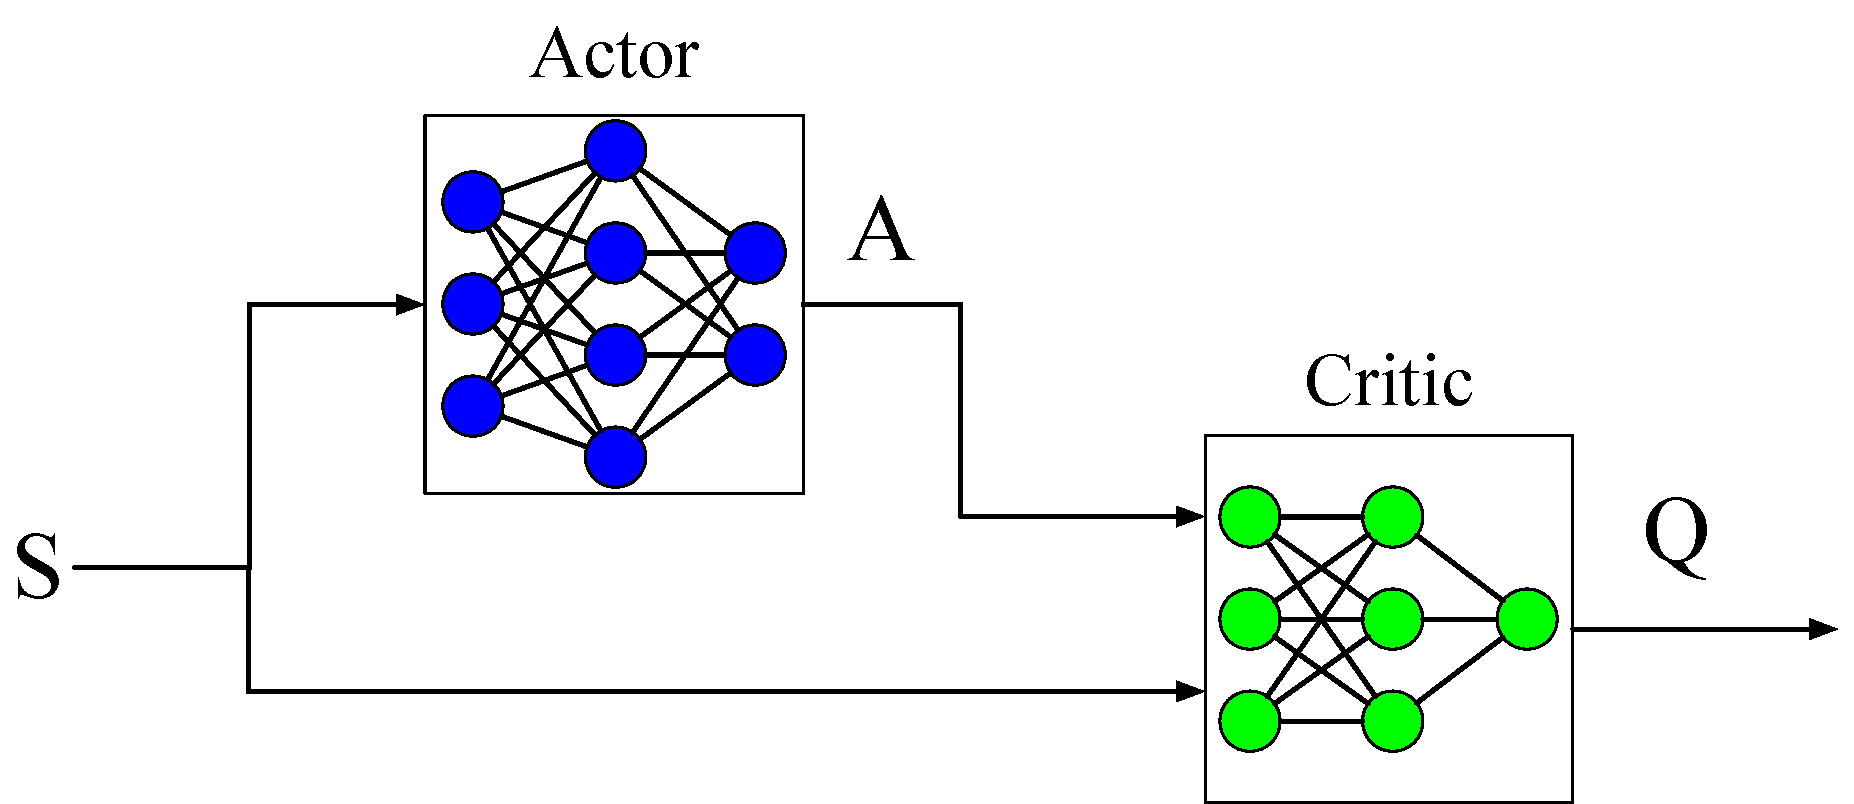
\includegraphics[width=7cm]{images/LookFurther/DDPG.pdf}}
\caption{Structure of DDPG.}
\label{ddpg}
\end{figure}

The DDPG algorithm has two different neural networks, actor networks $\mu(\textbf{x}_t|\theta^\mu)$ and critic networks $\nu(\textbf{x}_t,\textbf{a}_t|\theta^\nu)$, which are illustrated in Fig. \ref{ddpg}. $\theta^\mu$ and $\theta^\nu$ are the weights of the actor and critic network, respectively. Due to the non-linearity of the neural networks, the DDPG algorithm can deal with the continues states and continues actions, which are more realistic to autonomous systems. Actor network is used to yield a deterministic action value $\textbf{a}_t$, it takes the observation of environment as the inputs, and outputs the decided actions of the robot. Critic network is used to approximate $Q$ value, which is use to determine whether the state-action pair is good or not. It takes the observation from environment and the action value from actor networks, and then outputs the approximated $\nu(\textbf{x}_t,\textbf{a}_t)$ values. In the algorithm, the 
critic network is trained to minimise the loss function based on the stochastic gradient descent \cite{lillicrap2015continuous}:
\begin{equation}
    \mathcal{L}(\theta^\nu) = \mathbb{E}[(y_t - \nu(\textbf{x}_t,\textbf{a}_t|\theta^\nu))^2]
\end{equation}
where $y_t = r_t(\textbf{x}_t,\textbf{a}_t)+\gamma \nu(\textbf{x}_{t+1},\mu(\textbf{x}_t|\theta^\mu)|\theta^\nu)$ is the approximated $Q$ value based on current state $\textbf{x}_t$ and previous parameters $\theta^\mu, \theta^\nu$ of two neural networks.
%
The actor network is updated by the policy gradient with following equation \cite{lillicrap2015continuous}:
\begin{align}\label{DDPG}
    \nabla_{\theta^\mu}\mathcal{J}^{\theta^\mu} &= \mathbb{E}[\nabla_{\textbf{a}}\nu(\textbf{x},\textbf{a}|\theta^\nu)|_{\textbf{a}=\mu(\textbf{x}|\theta^\mu)}\nabla_{\theta^\mu}\mu(\textbf{x}|\theta^\mu)]
\end{align}

For the training, to breaking harmful correlations and learn from individual tuples for  multiple times, an experience replay buffer is applied. 
%Also, two additional neural networks, $\mu'(s|\theta^{\mu'})$ and $Q'(\textbf{x},\textbf{a}|\theta^{Q'})$, named target actor networks and target critic networks, are introduced to stabilize the training procedure \cite{van2016deep}.

For DDPG, a learned policy $\pi$ includes both actor network $\mu$ and critic network $\nu$. For some other DRL algorithms such as DQN, a learned policy $\pi$ may include only a  network $\mu$. 


\section{Sufficiency of Training Data}\label{sec:drlsufficiencytraining}

Theoretically, it is shown in \cite{DBLP:conf/alt/WeiszAS21} that the sample complexity, i.e., the number of  training-samples needed in order to successfully train a good model, is exponential with respect to either the input dimension or the finite horizon (of the sampled episodes). However, practical cases might not be as pessimistic as this looks like. 


Empirically, we can adapt the learning curve idea (which plots the test accuracy with respect to the training set size) to this context, and plot the curve to show the achieved performance as the function of the number of episodes played during the learning. Actually, the number of episodes played during the learning is a concept similar as the size of training dataset for the supervised training of classifiers, and we can define the achieved performance as e.g., expected reward over a number of rollouts. By tracing the curve, we will be able to know when additional episodes will not make a significant change to the training result. 


\section{Statistical Evaluation Methods}\label{sec:DRLevaluation}

Before introducing verification techniques which are usually of high computational complexity and hence are more suitable for safety-critical applications, we need some low-complexity evaluation methods to understand roughly how well a DRL algorithm works during training  and how well a trained DRL policy works in an environment. Those model evaluation methods for general machine learning models (such as ROC and PR curves) can still be applicable, but in this section we will introduce a few DRL specific evaluation methods. 



The below methods are all based on certain random variable $X$, and to track the trend and variance of $X$ in the training or test phase. 


\subsection*{Evaluation of DRL Training Algorithm}



In the training phase, the random variable $X$ can be e.g., per-epoch reward. Given a set of $X$'s values, they form a distribution. It is useful to use the dispersion (also called variability, scatter, or spread) of this distribution to understand if the training process goes well. The measurement of the dispersion of a distribution can be with a few indicators \cite{DBLP:journals/corr/abs-1912-05663} such as 
\begin{itemize}
    \item Interquartile Range (IQR). A distribution can be divided into 100 percentiles, denoted as $Q_1$, ..., $Q_{100}$, respectively. IQR can be defined as the difference between e.g., the 25th and 75th  percentiles, i.e., 
\begin{equation}
    \text{IQR}(X) = Q_{75}(X) - Q_{25}(X)
\end{equation}
    \item Conditional Value at Risk (CVaR). CVaR concerns the worst cases, by taking a weighted average of the worst-case losses in the left-most tail of the distribution of possible outcomes, formally 
    \begin{equation}
        \text{CVaR}_\alpha(X) = \mathbb{E}[X~|~X\leq \text{VaR}_\alpha(X)]
    \end{equation}
    where $\text{VaR}_\alpha$ (Value at Risk) is just the $\alpha$-th quantile (e.g., quartile, percentile, or decile) of the distribution of $X$.
\end{itemize}

Then, we may consider the change of the above indicators over the training time in a single training run or across different training runs. For a single training run, we can split it into a number of sliding widows and then collect $X$'s values from the sliding windows. When working with a set of different training runs, we can collect $X$'s values from those runs. 



\subsection*{Evaluation of DRL model}

Once there is a trained DRL policy, we can track its performance over a rollout by plotting the cumulative reward as a function of the number of steps. On such a plot, we may concern e.g., the slope, the minimum, and the zero-crossing (a point where the sign of the curve changes). 

Moreover, we can also consider $X$ as the performance over a set of rollouts, and use the IQR and CVaR to understand the dispersion of the distribution of $X$. 




\section{Safety Properties through Probabilistic Computational Tree Logic}\label{sec:DRLproperties}

%This section considers how to determine ${\cal M}^E(\pi,\textbf{x}_0)\models \phi$ when given a model ${\cal M}^E(\pi,\textbf{x}_0)$ and a property $\phi$. 

Probabilistic model checking \cite{kwiatkowska_probabilistic_2018} has been
used to analyse quantitative properties of systems across a variety of application domains. It involves the construction of a probabilistic model, e.g., DTMC or MDP, that formally represents the behaviour of a system over time. The properties of interest are usually specified with, e.g., LTL or PCTL. Then, via model checkers, a systematic exploration and analysis is performed to check if a claimed property holds. In this section, we adopt DTMC and PCTL whose definitions are as follows. %We remark that, the application of a policy $\pi$ over an MDP ${\cal M}^E$ induces a DTMC ${\cal M}^E(\pi,\textbf{x}_0)$. 

\begin{definition}[DTMC]
Let $AP$ be a set of atomic propositions. A DTMC is a tuple $(S,\textbf{x}_0,\textbf{P},L)$, where 
%\begin{itemize}
%\item 
$S$ is a (finite) set of states, $\textbf{x}_0\in S$ is an initial state, 
%\item 
$\textbf{P}:S\times S \rightarrow [0,1]$ is a probabilistic transition matrix such that $\sum_{s^{\prime}\in S}\textbf{P}(s,s^\prime)=1$ for all $s\in S$, and 
%\item 
$L:S\rightarrow 2^{AP}$ is a labelling function assigning  each state with a set of atomic propositions.
%from $AP$.
%\end{itemize}
\end{definition}
\begin{definition}[DTMC Reward Structure]
A reward structure for DTMC $D=(S,\textbf{x}_0,\textbf{P},L)$ is a tuple $r=(r_S, r_T)$ where $r_S:S\rightarrow \mathbb{R}_{\ge 0}$ is a state reward function and $r_T:S\times S \rightarrow \mathbb{R}_{\ge 0}$ is a transition reward function.
\end{definition}




\begin{definition}[PCTL]
The syntax of PCTL is defined by \emph{state formulae} $\phi$, \emph{path formulae} $\psi$ and \emph{reward formulae} $\mu$.
\begin{equation}\nonumber
\begin{aligned}
\phi &::= true \mid ap \mid \phi \wedge \phi \mid \neg \phi \mid {P}_{\bowtie p}(\psi) \mid {R}_{\bowtie q}^{r}(\mu)
\\
\psi &::= \next \: \phi \mid 
%\phi \: U^{\leq t} \: \phi \mid 
\phi \: U \: \phi 
\\
\mu &::= 
%I^{=t} \mid
C^{\leq t} \mid \eventually \: \phi
\end{aligned}
\end{equation}
where $ap \in AP, p\in [0,1], q\!\in \!\mathbb{R}_{\geq 0}, t\!\in\! \mathbb{N}$, $\bowtie \in \{<,\leq,>,\geq\}$ and $r$ is a reward structure. 
%
The temporal operator $\next$ is called ``next'', and  %$U^{\leq t}$ is called ``bounded until'' while 
$U$ is called ``until''. 
We write $\eventually \, \phi$ 
%as a syntax sugar 
for $true \, U \, \phi $, and call it ``eventually''. Operator 
%$I^{=t}$ represents the state reward at time step $t$---``instantaneous reward'', while 
$C^{\leq t}$ is ``bounded cumulative reward'', expressing the reward accumulated over $t$ steps.
%(when $t=\infty$, we write $C$ for short as the total reward accumulated indefinitely). 
Formula ${R}_{\bowtie q}^{r}(\eventually \, \phi)$ expresses ``reachability reward'', the reward accumulated up until the first time a state satisfying $\phi$. %\xiaowei{two $F$ formulas. to diamond}


%State formula $\phi$ is evaluated 
%to be either true or false in 
%on states.
%each state. 
Given $D=(S,\textbf{x}_0,\textbf{P},L)$ and $r=(r_S, r_T)$, the satisfaction of state formula $\phi$ on a state $s\in S$ is defined as:
%\begin{equation}
\begin{align}
s & \models true; \quad
s \models ap \, \Leftrightarrow\, ap \in L(s);\quad
s  \models \neg \phi \,\Leftrightarrow\, s \not\models \phi ; \nonumber
\\
s & \models \phi_1\wedge\phi_2 \, \Leftrightarrow\, s \models \phi_1 \text{ and } s \models \phi_2; \nonumber
\\
s & \models \mathcal{P}_{\bowtie p}(\psi) \,\Leftrightarrow\, Pr(s\models \psi)\bowtie p ; \nonumber
\\
s & \models \mathcal{R}_{\bowtie q}^{r}(\mu) \,\Leftrightarrow\, \mathbb{E}[rew^{r}(\mu)] \bowtie q, \nonumber
\end{align}
%\end{equation}

\noindent where $Pr(s\models \psi)\bowtie p $ concerns the probability of the set of paths that satisfy $\psi$ and start in $s$. Given a path $\eta$, if write $\eta[i]$ for its \textit{i}-th state and $\eta[0]$ the initial state, then
%
{\small
\begin{align}
%rew^{r}(I^{=t})(\eta)&=r_S(\eta[t]) \nonumber
%\\
rew^{r}(C^{\leq t})(\eta)&= \sum_{j=0}^{k-1}(r_S(\eta[j])+r_T(\eta[j],\eta[j+1])) \nonumber
\\
rew^{r}(\eventually\phi)(\eta)&=\begin{cases} \infty & \forall j \in \mathbb{N}(\eta[j] \not\models \phi) \\ rew^{r}(C^{\leq ind(\eta,\phi)})(\eta) & \text{otherwise}\end{cases} \nonumber
\end{align}}\normalsize
where $ind(\eta,\phi)=\min\{j|\eta[j] \models \phi\}$ denotes the index of the first occurrence of $\phi$ on path $\eta$.
Moreover, the satisfaction relations for a path formula $\psi$ on a path $\eta$ is defined as:
\begin{equation}\nonumber
\begin{aligned}
\eta & \models \next\phi \,\Leftrightarrow\, \eta[1] \models \phi 
\\
%\eta & \models \phi_1 \, U^{\leq t}\,\phi_2 \,\Leftrightarrow\,  \exists 0 \leq j \leq t \nonumber
%\\
% & \quad(\eta[j]\models \phi_2\wedge(\forall 0\leq k<j \; \eta[k]\models \phi_1))\\
\eta & \models \phi_1 \, U\,\phi_2 \,\Leftrightarrow\,  \exists j \geq 0 (\eta[j]\models \phi_2\wedge \forall k<j(\eta[k]\models \phi_1))
\end{aligned}
\end{equation}
\end{definition}

Very often, it is of interest to know the actual probability that a path formula is satisfied, rather than just whether or not the probability meets a required threshold since this can provide a notion of margins as well as benchmarks for comparisons following later updates. So, the \gls{PCTL} definition can be extended to allow \textit{numerical queries} of the form $\mathcal{P}_{=?}(\psi)$ or $\mathcal{R}^r_{=?}(\psi)$ \cite{kwiatkowska_probabilistic_2018}.
After formalising the system behaviors and properties in {DTMC} and {PCTL} respectively, 
%the verification focuses on checking of \textit{reachability} in a \gls{DTMC}. 
%That is, \gls{PCTL} expresses the constraints that must be satisfied, concerning the probability of, starting from the initial state, reaching some states labelled as, e.g., unsafe and success 
automated tools have been developed to solve the verification problem, e.g., PRISM \cite{kwiatkowska_prism_2011} and STORM \cite{dehnert_storm_2017}.
%\footnote{Since each tool of its current version (at the time of writing) has some limitations, e.g., PRISM cannot check conditional probabilities while STORM cannot check \gls{LTL}-style properties.}.
%which employ a symbolic model checking algorithm to calculate the probability that a path formulae is satisfied. 
%
We remark that, PCTL can be utilised to describe safety-related properties for e.g., the robot navigation example  Example~\ref{example:robotnavigation} as discussed in \cite{DBLP:journals/corr/abs-2109-06523}. 


In the following sections, we will discuss several instantiations of the DTMC  as ${\cal M}^E(\pi,\textbf{x}_0)$ (Section~\ref{sec:DRLverification}), ${\cal M}^E(\pi,\textbf{x}_0,\mathcal{C})$ (Section~\ref{sec:DRLRobustnessverification}), ${\cal M}^E(\pi,\mathcal{C}(\textbf{x}_0))$ (Section~\ref{sec:verificationtemporalDRLrobustness}), and  ${\cal M}^{E_1\times E_2}(\pi,(\textbf{x}_0,\textbf{x}_0))$ (Section~\ref{sec:verificationsim2real}), respectively. 

%It is worth noting that both \gls{DTMC} and \gls{PCTL} can be augmented with rewards/costs \cite{filieri_probabilistic_2013}, which can be used to model, e.g. the energy consumption of \gls{RAS} \cite{zhao_toward\textbf{x}_2019}. As readers will see, we also utilise rewards/costs in formalising some of our properties, e.g., resilience.

\begin{comment}%% If we have the space to present the actually PRISM model, we then need to insert back the following description.
In general, a PRISM module contains a number of local variables which constitute the state of the module. The transition behaviour of the states in a module is described by a set of commands which take the form of:
\begin{equation}
    [Action] \: Guard \rightarrow Prob_1 : Update_1 + ... + Prob_n : Update_n ; \nonumber
\end{equation}
As described by the PRISM manual\footnote{https://www.prismmodelchecker.org/manual/}, the guard is a predicate over all the variables (including those belonging to other modules. Thus, together with the action labels, it allows modules to synchronise). Each update describes a transition which the module can make if the guard is true. A transition is specified by giving the new values of the variables in the module, possibly as a function of other variables. Each update is also assigned a probability (in our \gls{DTMC} case) which will be assigned to the corresponding transition. 
\end{comment}



\section{Verification of Policy Generalisation}\label{sec:DRLverification}


Although at any specific time a DRL agent with actor network $\mu$ -- like the classifier -- also returns an action $\mu(\textbf{x})$ according to the state $\textbf{x}$, the correctness of the action $\mu(\textbf{x})$ is not solely dependent on the state $\textbf{x}$. Instead, considering its training mechanism, the correctness of the action at any specific time depends on the expected long-term accumulated rewards. For this reason, the verification of a DRL agent also needs to consider not only the current state but also the long-term rewards (and therefore the future states). Therefore, to understand if a learned policy $\pi$ works well in an environment MDP ${\cal M}^E$, we can conduct probabilistic model checking on their induced DTMC ${\cal M}^E(\pi,\textbf{x}_0)$, where $\textbf{x}_0$ is an initial state of ${\cal M}^E$. This enables the analysis of various properties that can be expressed with PCTL. 

When the exact construction of the DTMC ${\cal M}^E(\pi,\textbf{x}_0)$ is hard (due to e.g., some components of the environment ${\cal M}^E$ is unknown, or the policy network is too big for analysis), as discussed in \cite{DBLP:journals/corr/abs-2109-06523}, we can approximate it from a set of sampled trajectories. 

Actually, due to the high-dimensionality of the underlying control problem and the continuity of some state and observable variables, it is unlikely that we can construct a DTMC that is exactly the application of policy $\pi$ to MDP ${\cal M}^E$. Certain abstraction techniques \cite{clarkebook} will be needed, for example, we consider predicate abstraction, where the DTMC's state space is constructed from a given set of predicates over MDP's  state variables, as we will discuss below. 

\subsection*{Construction of a DTMC Describing the Failure Process}\label{sec:DTMCconstruction}

We consider the execution of the policy $\pi$ in an environment. For simplicity, we only differentiate the environments with a disturbance level that the robot's sensory input may be subject to, and assume that the disturbance level follows a distribution $\mathcal{N}(0,\sigma)$.
Now, as stated in Section~\ref{sec:mdp}, given an MDP ${\cal M}^\sigma$ (based on a disturbance $\mathcal{N}(0,\sigma)$) and a DRL policy $\pi$, there is a trajectory distribution $\rho^{\pi,\sigma}(\zeta)$.  
Based on the \textit{dynamics of risk-levels} in $\rho^{\pi,\sigma}(\zeta)$,  
%during the \gls{RAS} mission, 
we 
%first 
can define a DTMC, 
%structure 
%for the proposed assessment framework, 
as shown in Fig. \ref{dtmc}. It consists of a ``negligible-risk'' state $s_N$, a catastrophic failure state $s_C$, and several states $s_{B_i}$ representing different levels of ``benign failures''.
%(risky states that might lead to a catastrophic failure later). 
%TODO: remove all \vspace once accepted...
%\vspace{-1mm}
\begin{figure}[htbp]
\centerline{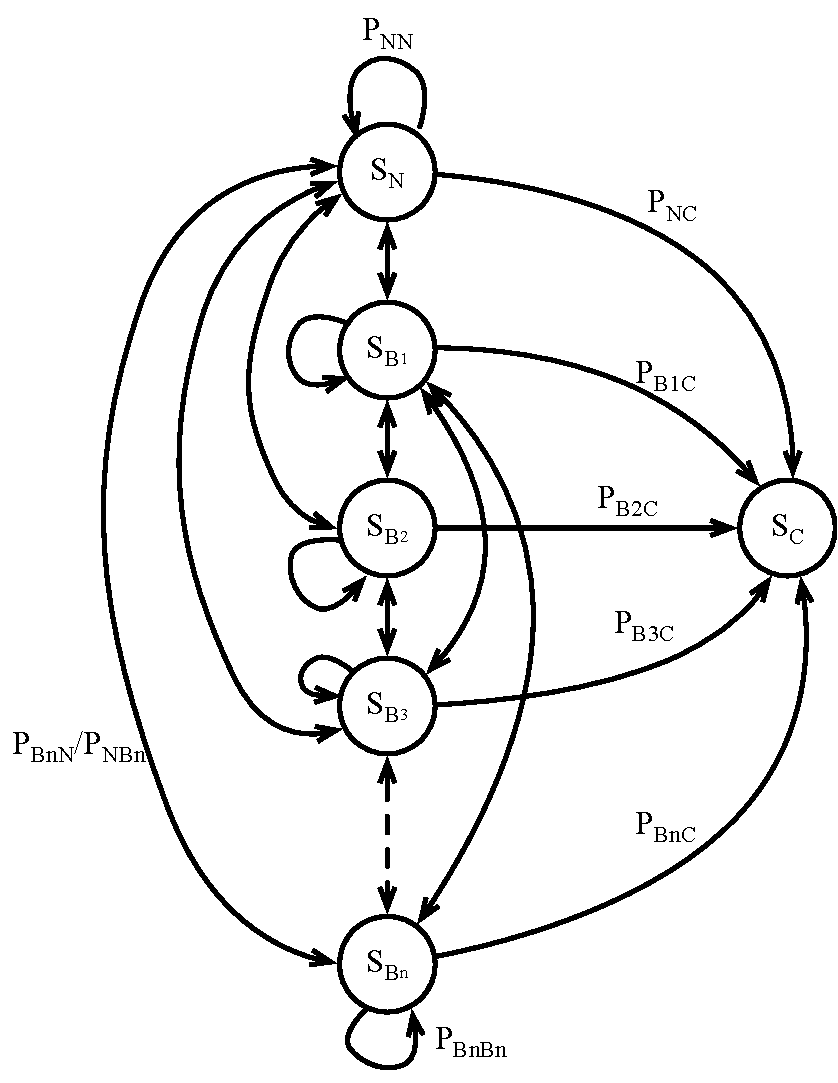
\includegraphics[width=0.4\textwidth]{images/LookFurther/DTMC.pdf}}
\centering
%\vspace{-2mm}
\caption{The failure process DTMC based on risk-levels.}
\label{dtmc}
\end{figure}%\vspace{-2mm}

%Given a trained
%/frozen 
%\gls{DRL} policy, statistical testing is conducted to test the \gls{RAS} with different disturbance-levels (representing noisy environmental factors), yielding a set of \textit{mission trajectories}. Note, each
%We can use statistical testing to get a finite set of trajectories from $\rho^{\pi,\sigma}(\zeta)$. 
Each trajectory is a sequence of successive states %(or path) 
from the initial state to the end state of a DRL episode. First, we map each state in the trajectories to one of the states describing the failure process (i.e., $s_N$, $s_C$, and $s_{B_i}$). Second, we may conduct statistical analysis on the frequency of transitions between $s_N$, $s_C$, and $s_{B_i}$, based on which we 
%invoke estimators to 
estimate their corresponding transition probabilities. Finally, we construct the failure process DTMC with the defined structure and the estimated transition probabilities.
%(which is encoded later by some formal language and fed into model checkers). 
To be exact, we describe the 3 main steps above as what follows.
%The \gls{DRL} policy is abstracted into the induced DTMC, and the normal and safe states are modelled in the non-risky route state. In the proposed DTMC framework, each state can transit into one or more unsafe states with different probabilities, e.g. in a safe driving state $s_G$, the autonomous robot may fall into an unsafe state $B_3$ if there is a suddenly injected obstacle. We divide the unsafe states into several different levels, $B_1, B_2, \cdots, B_n$ to reveal different failure levels. The far from the safe states, the higher the possibility of mission failure, but none of the benign failures will cause any catastrophic damage to the autonomous robot.



\subsubsection{Mapping MDP States onto DTMC States}

% 
%Without loss of generality, 
%in this paper, 
First of all, every state in the DTMC (cf. Fig.~\ref{dtmc}) is associated with a risk level. Specifically, $s_N$ is the negligible-risk state, $s_C$ is the catastrophic
failure state, and $s_{B_i}$ are benign failure states such that the risk on $s_{B_i}$ is higher than on $s_{B_j}$ if $i>j$. 

Now, to map $\mathcal{S}$ (the states on the trajectories) onto $S$ (the states on the DTMC), we define a measure of risk based on the distance of the robot to obstacles. 
%
For instance, $s_N$ suggests that the robot is 3+ metres away from the obstacle, $s_{B_1}$ suggests 2-3 metres away, 
$s_{B_2}$ suggests 1-2 metres away, etc.  %and  
%but within 3m 
%represents state  
%(similarly for $s_{B2}$, etc), 
%and.
Moreover, catastrophic failure $s_C$ is defined as the robot terminated unexpectedly by a non-recoverable failure.  The determination of the risk levels for states in $\mathcal{S}$ can be done by evaluating the sensory input. We remark that, this is a predicate abstraction where $s_N$, $s_{B_1}$, $s_{B_2}$, and $s_C$ can be seem as predicates such that only one predicate can be True on any MDP state. 

%for every state $s\in \mathcal{S}$, we have a measure of risk. W.l.o.g.,
%our measure of risks
%we define the measure based on the distance to obstacles. 

\iffalse

\begin{definition}[Negligible-Risk State]
A state $s$ is mapped onto the negligible-risk state $s_N$  if the measure of risk on $s$ is below a pre-specified safe threshold.
%is defined as an .
\end{definition}
\begin{definition}[Benign Failure State]
A state, denoted as $s_{B_i}$, in which the measure of risk is above the safe threshold but lower than a specified level $B_i$ (while the \gls{RAS} mission is still ongoing) is defined as a benign failure state.
\end{definition}
\begin{definition}[Catastrophic Failure State]
A state, denoted as $s_{C}$, in which we observe the \gls{RAS} mission is terminated unexpectedly by a non-recoverable catastrophic failure is defined as a catastrophic failure state.
\end{definition}
\fi

%\noindent 
\begin{definition}[Negligible-Risk Route]
Given an MDP ${\cal M}^\sigma$ and a DRL policy $\pi$, a \textit{negligible-risk route} is defined as a mission trajectory in $\rho^{\pi,\sigma}(\zeta)$ that contains only $s_N$ states.
%the non-risky route in a \gls{RAS} environment. The \textit{Non-Risky Route} is the safest route, but it may not be the route with the highest reward under the concept of \gls{DRL}. \xiaowei{I believe we need a formal definition on the ``non-risky route''. Given a policy, there might not exist a path which stays on $s_G$. }
\end{definition}

 We remark that,
\iffalse
: (i) Although in some extreme 
cases 
%environments
with high-level of disturbance the negligible-risk route may not exist in practice, there is always a negligible-risk route in theory (potentially with 
%extreme 
small probabilities); (ii) The 
\fi
the negligible-risk route is not necessarily the optimal route achieving the highest reward,
%in the training of the DRL, 
rather it 
only depends on the 
%observations of the 
risk-levels during the RAS mission.



\subsubsection{Estimating Transition Probabilities}

We can collect a set of mission trajectories by conducting 
%After the 
statistical testing (the simple Monte Carlo sampling in our case) on $\rho^{\pi,\sigma}(\zeta)$. 
%Given a trajectory, mapping each of its state to one of the states describing the failure process will result a sequence of states consisted of $s_N$, $s_C$ and $s_{B_i}$, and thus transitions among them as well. 
Then, all mission trajectories collectively can be transformed into a 
%large 
set of transitions, based on which we build a transition matrix to record the statistical data as follows:
\begin{table}[h!]
\centering
\begin{tabular}{l|lllll}
         & $s_N$       & $s_{B_1}$  & ... & $s_{B_m}$      & $s_C$         \\ \hline
$s_N$    & $n_{1,1}$   & $n_{1,2}$ & ... & $n_{1,m+1}$   & $n_{1,m+2}$   \\
$s_{B_1}$ & $n_{2,1}$   & $n_{2,2}$ & ... & ...           & ...           \\
...      & ...         & ...       & ... & ...           & ...           \\
$s_{B_m}$ & $n_{m+1,1}$ & ...       & ... & $n_{m+1,m+1}$ & ...           \\
$s_C$    & $n_{m+2,1}$ & ...       & ... & ...           & $n_{m+2,m+2}$
\end{tabular}
\end{table}
\newline
where $n_{1,1}$ records the number of transitions from $s_N$ to $s_N$, and so on.
%so forth. 
%While 
$m$ is the number of levels of benign failures (that varies case by case depends on the application-specific context, e.g., we choose $m=3$ in our 
%later 
experiments).

%Let us denote 
Let the transition probability matrix of the failure process DTMC be $\textbf{P}_1=(p_{ij})\in [0,1]^{(m+2)\times (m+2)}$. 
In a DTMC, given a current state $i$, the transition to a next state follows a \textit{categorical distribution}. Due to the Markov property, the categorical distributions of each state are \textit{independent}. Hence, as we observe repeated outgoing transitions from state $i$, the repeated categorical process follows a \textit{multinomial distribution}. For the $i$-th row of $\textbf{P}_1$, the likelihood function $\mathcal{L}$ is (by omitting the combinatorial factor):
\begin{equation}
\label{eq_likelihood_row_i}
\mathcal{L}(  p_{i,1},\dots,p_{i,m+2} \mid n_{1,1},\dots,n_{1,m+2})=\prod_{j=1}^{m+2} p_{i,j}^{n_{i,j}}
\end{equation}
%\xiaowei{I don't quite understand this likelihood function. }

Upon establishing the likelihood function, many existing estimators can be invoked for our purpose, such as the basic Maximum Likelihood Estimation (MLE) and Bayesian estimators \cite{epifani_model_2009}. While more advanced estimators can be easily integrated in our proposed framework, we only present the use of MLE in this paper for brevity:
\begin{equation}
\label{eq_mle_tranprob}
    \hat{p}_{i,j}=\frac{n_{i,j}}{\sum_{j=1}^{m+2} n_{i,j}}
\end{equation}
It is known that MLE is an unbiased estimator 
%in this case 
\cite{epifani_model_2009}, while the uncertainty in the estimates is captured by the variance that depends on the number of samples. There are also means for calculating $(1-\alpha)$ confidence intervals of the verification results, given the observations on the frequencies between states (exactly as our statistical data $n_{i,j}$). Such result may in turn determine the required number of samples $n_{i,j}$ given a required say 95\% confidence level for the final verification results. Although we did not calculate the confidence interval to determine the sample size in this paper, we instead choose a sample size in our later experiments that is sufficiently large to show a converging trend of the verification results.
%(cf. Section~\ref{sec.5.3}). 

\subsubsection{Construction of Failure Process DTMC}
\label{sec_formalise_DTMC}
%Let $AP=\{term, p_G, p_{B^1},..., p_{B^n}\}$. From a trajectory distribution $\rho^\pi(\zeta)$ induced from a policy $\pi$ and an MDP $\cal{M}$,  we  construct a DTMC $(S,s_G,\textbf{P},L)$ such that $S=\{s_G, s_{B^1},...,s_{B^n}, s_C\}$,  $term \in L(s_C)$, and $p_{B^i}\in L{s_{B^i}}$ for $i\in \{1..n\}$. The probabilistic transition $\textbf{P}$ is defined as $\textbf{P}(s_G,s_1)=$
%\xingyu{double check with Xiaowei...}

The failure process DTMC is the product of two DTMCs, $M_1$ and $M_2$, via the synchronisation of the transition actions.

Let $AP_1=\{crash, neg\_risk, risk\_B_1,\cdots, risk\_B_n\}$, and 
%From a trajectory distribution $\rho^\pi(\zeta)$ induced from a policy $\pi$ and an MDP $\cal{M}$, 
we construct the first DTMC $M_1=(S,s_N,\textbf{P}_1,L_1)$ where
\begin{itemize}
    \item $S=\{s_N, s_{B_1},\dots,s_{B_n}, s_C\}$,
    \item Each entry $p_{i,j}$ of 
%the probabilistic transition matrix 
$\textbf{P}_1$ is defined as Eqn.~\eqref{eq_mle_tranprob}, and 
    \item $neg\_risk \in L_1(s_N)$,  $risk\_B_i\in L_1(s_{B_i})$ for $i\in \{1..n\}$, and
     $crash \in L_1(s_C)$.
\end{itemize}    We also define a reward structure 
%for this DTMC 
%as
{``deviation''}$=(r_S,r_T)$ with
\begin{itemize}
    \item $r_S(s_N)=0$,
    \item $r_S(s_C)=0$,
    \item $r_S(s_{B_i})=d_i$ (where $d_i$ is the deviation from $s_N$ to $s_{B_i}$), and 
    \item $r_T(s1,s2)=0$ for all $s1, s2 \in S$.
\end{itemize} 


%Since the properties 
%of our interest 
%may depend on %in which 
%the stage the \gls{RAS} is during the mission, 
Moreover, we %also 
%formalise 
need a ``mission stage DTMC'' (for simplicity, we only consider two stages---mission terminated or not). Let $AP=\{progressing,terminated\}$, we construct
%a DTMC 
$M_2=(K,k_0,\textbf{P}_2,L_2)$ with
\begin{itemize}
    \item $K=\{k_0,k_1\}$,
    \item $progressing \in L_2(k_0)$ and $terminated \in L_2(k_1)$, and 
    \item The transition probabilities $\textbf{P}_2$ are $p_{k_0,k_1}=\frac{1}{l_{mis}},p_{k_0,k_0}=1-\frac{1}{l_{mis}}, p_{k_1,k_1}=1$ and $p_{k_1,k_0}=0$, where $l_{mis}$ is a constant representing the expected mission length (number of transitions) obtained from the testing data.
\end{itemize}  We also define a reward structure for this DTMC:  {``step''}$=(r_S,r_T)$ with
\begin{itemize}
    \item $r_T(k_0,k_0)=1$,
    \item $r_T(k_0,k_1)=1$, and 
    \item $r_S(k)=0$ for all $k \in K$.
\end{itemize}  

%In later experiments, 
Finally,  
%further 
%encode the two DTMCs in the 
%for model checking, 
we encode the failure process DTMC with PRISM model checker \cite{kwiatkowska_prism_2011}.

\section{Verification of State-Based Policy Robustness}\label{sec:DRLRobustnessverification}

The verification in Section~\ref{sec:DRLverification} mainly concerns whether a learned policy works well in an environment. It actually computes the generalisation ability of the policy in the environment, considering the fact that the policy might not be trained on all paths of the DTMC but is expected to generalise well. Nevertheless, there are other safety properties to be considered. In this section, we consider temporal properties over the state-based robustness. 

For state-based robustness, we concern the the robustness of the policy network (and other supplementary network such as the critic network of DDPG) on individual states. Therefore, temporal properties over the state-based robustness  measure the  dynamics of such robustness of the neural networks when DRL agent interacts with the environment. Actually, state-based robustness is mainly due to the existence of observation noises (from e.g., noisy sensor reading), and we assume that such noise only influences the current state. We will discuss in the next section (Section~\ref{sec:verificationtemporalDRLrobustness}) the case where the noise at a state may influence the future states. 

Formally, to work with state-based policy robustness, we need to lift the model  ${\cal M}^E(\pi,\textbf{x}_0)$ into ${\cal M}^E(\pi,\textbf{x}_0, \mathcal{C})$ to consider the constraint $\mathcal{C}$ on the noise. 

\subsection*{Modelling Noise}




Usually, the constraint $\mathcal{C}(\textbf{x})$ expresses the neighborhood of a state $\textbf{x}$. A neighborhood can be e.g., a distance norm based neighborhood as  \begin{equation}
     \{ \textbf{x}' ~|~ ||\textbf{x} - \textbf{x}'||_p \leq d\},
\end{equation}
a Zonotope expressed as a Minkowski sum of a set of planes, or any other topological shape. Recall that, we use $||\cdot||_p$ to express the $L_p$ norm of a vector for $p\geq 0$. 

An immediate impact of the state-based noise is, instead of having a deterministic action and a single approximated Q value (when given a critic network), there are a set of possible actions and a set of possible approximated Q values. 


\subsection*{Example Properties}

We may consider a few example properties in the following, to quantify the uncertainty incurred by the noise. 

\begin{example}\label{example:robustDRLproperties}
We may write 
property \begin{equation}
    \mathcal{P}_{\leq 0}~\eventually~(\textbf{a}\in \mathcal{A}_{valid})
\end{equation}
to express that it is almost sure that some action $\textbf{a}$ is never activated, where $\mathcal{A}_{valid}$ is the set of actions that are possible at the current state, subject to the noise.  Moreover, we may write 
\begin{equation}
    \mathcal{P}_{\leq 0}~\eventually~(r > c)
\end{equation}
to express that the predictive Q value $r$ (output by the critic network) is always no greater than $c$, subject to the noise at the current state. 
\end{example}

For the remaining of this section, we will discuss how to extend the  DTMC ${\cal M}^E(\pi,\textbf{x}_0)$ into ${\cal M}^E(\pi,\textbf{x}_0,\mathcal{C})$ to work with the properties as in Example~\ref{example:robustDRLproperties}. Actually, we need to expand the set $Prop$ of atomic propositions to include atomic propositions such as $\textbf{a}\in \mathcal{A}_{valid}$ and $r > c$. For this, we need to change the state space from $\mathcal{S}$ to $\mathcal{S}\times \mathcal{P}(\mathcal{S})$, so that we can compute e.g.,  $\mathcal{A}_{valid}$,  $r_{min}$, and $r_{max}$ over expanded states, where $[r_{min},r_{max}]$ is the reachable range of the predictive Q value $r$. 

\subsection*{Expansion of State Space}

Comparing with ${\cal M}^E(\pi,\textbf{x}_0)$, the new model ${\cal M}^E(\pi,\textbf{x}_0, \mathcal{C})$ has an expanded state space $\mathcal{S}\times \mathcal{P}(\mathcal{S})$ such that each state $\textbf{x}$ is now attached with a noise neighborhood $\mathcal{C}(\textbf{x})$. The transition relation depends only on the first element, i.e., on the state $\textbf{x}$, so it can be easily obtained from the transition relation of the model ${\cal M}^E(\pi,\textbf{x}_0)$. Another expansion is on the atomic propositions, which as explained will include some additional atomic propositions as in Example~\ref{example:robustDRLproperties}. 

\subsection*{Evaluation of Atomic Propositions}

Considering a typical DRL agent which has two neural networks $\mu: \mathcal{S}\rightarrow \mathcal{A}$ and $\nu: \mathcal{S}\times \mathcal{A} \rightarrow \mathcal{N}$, representing the actor and the critic agents, respectively. Intuitively, $\mu(\textbf{x})$ returns the action $\textbf{a}$ that needs to be taken on a state $\textbf{x}$, while $\nu(\textbf{x},\textbf{a})$ returns the predictive Q value of taking action $\textbf{a}$ on state $\textbf{x}$. Assume that we have a verification tool $g$ that, given $\mu$ and a constraint $\mathcal{C}(\textbf{x})$ in $\mathcal{S}$, outputs an (over-approximated) reachable set in 
$\mathcal{A}$. That is, we can have 
\begin{equation}\label{equ:reachableactions}
    g(\mu,\mathcal{C}(\textbf{x})) 
\end{equation}
as the reachable set of actions when given a set of states expressed with constraint $\mathcal{C}(\textbf{x})$. With this, we can determine $\textbf{a}\in \mathcal{A}_{valid}$ by knowing whether $\textbf{a}\in g(\mu,\mathcal{C}(\textbf{x})) $.
Such verification tool is available \cite{HUANG2020100270} in previous works \cite{RHK2018,wu2018game,10.1007/978-3-030-32304-2_15}. Moreover, we can compute 
\begin{equation}\label{equ:reachablestates}
    g(\nu,\mathcal{C}(\textbf{x})\times g(\mu,\mathcal{C}(\textbf{x})))
\end{equation}
as the range of predictive Q value, and hence know the values $r_{min}$ and $r_{max}$. Based on them, we can determine if $r>c$.  



%Given a set of observations $\textbf{X}$, we write $\eta(\textbf{X})$ for the minimum shape that contains the set $\textbf{X}$  such that $\textbf{X}\subseteq \eta(\textbf{X})$, where $\eta$ can be e.g., \textbf{Box} and \textbf{Zonotope}, as discussed above.

\subsection*{Probabilistic Model Checking Lifted with New Atomic Propositions}



%In the following, depending on whether learning an environment agent is possible, we have two different ways of computing 

%verification approaches to work with a PCTL safety property \begin{equation}
%    \mathcal{P}_{\geq 1}(true \: U \: p)
%\end{equation} 
%which expresses the almost sure reachability of states satisfying $p$. Note that, $true \: U \: p$ denotes the finite reachability of $p$. 

%\subsection*{Learning Environment Agent}


As explained above, when using neighborhood $\mathcal{C}(\textbf{x})$ to express adding noise to the state $\textbf{x}$, we can lift the DTMC ${\cal M}^E(\pi,\textbf{x}_0)$ into ${\cal M}^E(\pi,\textbf{x}_0, \mathcal{C})$ by associating each state $\textbf{x}$ with a neighborhood $\mathcal{C}(\textbf{x})$. Then, the probabilistic model checking proceeds the same as in Section~\ref{sec:DRLverification} with the  additional consideration of the  neighborhood $\mathcal{C}(\textbf{x})$ on every state as well as the above-mentioned evaluation of atomic propositions. 



\iffalse

To conduct verification, we may have an environment agent $E:\mathcal{S}\times \mathcal{A} \rightarrow \mathcal{P}(\mathcal{S})$, which returns a distribution of next states when given an action on the current state. Such environment can be learned as in \cite{DBLP:journals/corr/abs-1803-10122}. Similar as Equation (\ref{equ:reachableactions}), we have 
\begin{equation}
    g(E, \mathcal{C} \times \mathcal{C}_{\mathcal{A}}) 
\end{equation}
as the reachable set of next states when given a set of states expressed with $\mathcal{C}$ and a set of actions expressed with $\mathcal{C}_{\mathcal{A}}$. 

Based on the above, once we have $E$ and $\mu$, and a set $\mathcal{C}$ of constraints on the current states, we can compute  
\begin{equation}
    \mathcal{C}' = g(E, \mathcal{C} \times g(\mu,\mathcal{C}))
\end{equation}
as the  set of reachable next states. This step can be repeated until obtaining  $\mathcal{C}^{(k)}$ after $k>1$ steps. We can then check whether $(\mathcal{C},\mathcal{C}^{(k)})$ satisfies the constraint $\mathcal{C}$ as defined with e.g., PCTL formulas. 

%\paragraph{Which property to verify?} We consider PCTL property which concerns the expected reward upon $\mu$. 

%\paragraph{Is this a challenging problem?} 

%There are two challenging issues. The first is the lack of environment model. The second is the computation of reachable actions. 

\fi

\section{Verification of Temporal Policy Robustness}\label{sec:verificationtemporalDRLrobustness}

The state-based policy robustness, as discussed in Section~\ref{sec:DRLRobustnessverification}, concerns the dynamics of the robustness of the policy network $\mu$ (and the critic network $\nu$) on individual states of a path.  When the states $\textbf{x}_k$ and $\textbf{x}_{k+1}$ are known, the robustness on state $\textbf{x}_k$ cannot influence the robustness on $\textbf{x}_{k+1}$. This is a simplistic assumption, but can be arguably unrealistic. In this section, we consider a more complex setting about the temporal evolution of robustness, i.e., the robustness on state $\textbf{x}_k$ may influence the robustness of later states $\textbf{x}_{k+1}, \textbf{x}_{k+2}, ...$.  

%When learning an environment agent is infeasible, we can consider an alternative approach. 
To work with temporal evolution of robustness, we cannot re-use the DTMC ${\cal M}^E(\pi,\textbf{x}_0)$. Instead, we need to construct a new Kripke structure \cite{clarkebook} ${\cal M}^E(\pi,\mathcal{C}(\textbf{x}_0))=(S,s_0,T,L)$ from the environment MDP ${\cal M}^E$, the DRL policy $\pi$, the initial state $\textbf{x}_0$, and the noise constraint $\mathcal{C}$. Also, we do not work wih the probabilistic logic PCTL because the transition relation $T$ in $M$ is non-probabilistic, and will work with a non-probabilistic temporal logic LTL. 

\subsection*{State Space}

Given a set of MDP states $\textbf{X}$, we write $\eta(\textbf{X})$ for the minimum polytope that contains the set $\textbf{X}$, i.e., $\textbf{X}\subseteq \eta(\textbf{X})$, where $\eta$ can be e.g., \textbf{Box} and \textbf{Zonotope}, as discussed above. Intuitively, $\eta(\textbf{X})$ is an over-approximation of $\textbf{X}$. Let $S$ of ${\cal M}^E(\pi,\mathcal{C}(\textbf{x}_0))$ be the set of states such that every state $s$ is a polytope $\eta(\textbf{X})$.  The function $\eta$ is used to keep all the states in ${\cal M}^E(\pi,\mathcal{C}(\textbf{x}_0))$ as the same polytope shape, to make the state space manageable. With this definition of states $S$, the initial state $
s_0= \eta(\mathcal{C}(\textbf{x}_0))$ is the polytope containing the noise neighborhood of the initial observation $\textbf{x}_0$. 

\subsection*{Transition Relation}

First of all, we need two supplementary functions. 
The first function $h_1$ is, given a constraint $\mathcal{C}$, to split $\mathcal{C}$ into a set of constraints, i.e.,  
\begin{equation}
    h_1(\mathcal{C},g,\mu) = \{\mathcal{C}^{\textbf{a}_1}, ..., \mathcal{C}^{\textbf{a}_m}\}
\end{equation}
such that $\mathcal{C} = \mathcal{C}^{\textbf{a}_1}\cup ... \cup \mathcal{C}^{\textbf{a}_m}$ and, for all $1\leq i\leq m$, $g(\mu,\mathcal{C}^{\textbf{a}_i})=\{\textbf{a}_i\}$. Intuitively, after splitting, all states in a constraint $\mathcal{C}^{\textbf{a}_i}$ take the same action $\textbf{a}_i$. We write $a(\mathcal{C}^{\textbf{a}_i})=\textbf{a}_i$. The second function $h_2$ is, given constraints $\mathcal{C}$ and an action $\textbf{a}$, to return the set of next states, i.e.,  
\begin{equation}
    h_2(\mathcal{C},\textbf{a}) =  \bigcup_{\textbf{x}\in \mathcal{C}} support(\mathcal{P}(\textbf{x},\textbf{a})) 
\end{equation}
where $\textbf{x}\in \mathcal{C}$ means that the state $\textbf{x}$ satisfies the constraint $\mathcal{C}$, and $support(D)$ returns the support of a distribution $D$. We recall that $\mathcal{P}(\textbf{x},\textbf{a})$ is the probabilistic transition function of ${\cal M}^E$. We remark that, $h_1$ can be obtained by applying binary search together with the verification tool $g$, and $h_2$ can be obtained by a genetic algorithm to search for a convex hull over the next states. 

Based on $h_1$ and $h_2$, we can construct the transition relation $T$ of ${\cal M}^E(\pi,\mathcal{C}(\textbf{x}_0))$. For every suitable polytope $\mathcal{C}$, we let 
\begin{equation}
    (\mathcal{C},\mathcal{C}')\in T\text{ for every }\mathcal{C}'\in \{\eta(h_2(\mathcal{C}^{\textbf{a}},\textbf{a}))~|~\mathcal{C}^{\textbf{a}} \in h_1(\mathcal{C},g,\mu)\}.
\end{equation} Note that, with this construction, we assume that the noise is only from the initial state, without having any additional noise in the later steps. If we need to consider additional noise for every step, we may replace the set $\{\eta(h_2(\mathcal{C}^{\textbf{a}},\textbf{a}))~|~\mathcal{C}^{\textbf{a}} \in h_1(\mathcal{C},g,\mu)\}$ with $\{\eta(\mathcal{C}(h_2(\mathcal{C}^{\textbf{a}},\textbf{a})))~|~\mathcal{C}^{\textbf{a}} \in h_1(\mathcal{C},g,\mu)\}$, i.e., every input subset $h_2(\mathcal{C}^{\textbf{a}},\textbf{a})$ is added with noise represented with the constraint $\mathcal{C}$.


\subsection*{LTL Model Checking}

The labelling function $L$ of ${\cal M}^E(\pi,\mathcal{C}(\textbf{x}_0))$ is the same as the one in the DTMC ${\cal M}^E(\pi,\textbf{x}_0)$ for atomic propositions such as $\textbf{a}\in \mathcal{A}_{valid}$ and $r > c$. The Kripke structure ${\cal M}^E(\pi,\mathcal{C}(\textbf{x}_0))$ is non-probabilistic. Therefore, we can apply LTL model checking~\cite{clarkebook} to understand the qualitative properties such as 
\begin{equation}
    \neg \eventually\neg ~(\textbf{a}\notin \mathcal{A}_{valid})
\end{equation}
which expresses that action $\textbf{a}$ will never occur, and 
\begin{equation}
    \neg \eventually\neg ~(r \leq  c)
\end{equation}
which expresses that the predictive Q value $r$ is always no greater than $c$. 

\iffalse

Now, given a constraint $\mathcal{C}$ on the current states, we determine the safety of   $\mathcal{C}$, written as $\mathcal{C}\models \mathcal{C}$, with 
\begin{equation}\label{equ:spliting}
    \bigwedge_{\mathcal{C}\in h_1(\mathcal{C},g,\mu)} h_2(\mathcal{C},a(\mathcal{C}))\models \mathcal{C}
\end{equation}
Note that, Equation (\ref{equ:spliting}) is a recursive definition, i.e., $h_2(\mathcal{C},a(\mathcal{C}))\models \mathcal{C}$ can also be computed in this way. By recursively computing Equation (\ref{equ:spliting}) for $k$ steps, we can have the verification result. 



\fi



\section{Addressing Sim-to-Real Challenge}\label{sec:verificationsim2real}

Considering the lack of real-world training data for DRL agents, it is a common practice to train a DRL policy in a simulation environment and then consider its application in real-world settings by transferring the knowledge and adapting the policy. More and more high-fidelity simulation platforms such as  AirSim \cite{10.1007/978-3-319-67361-5_40}, CARLA~\cite{DBLP:journals/corr/abs-1711-03938}, and RotorS~\cite{Furrer2016} have been made available, in order to reduce the gap between simulation and reality.  Nevertheless, the gap exists and technical means to detect and reduce the gap are still needed. Typical methods to reduce the gap during training include e.g., adding perturbances to the environment \cite{DBLP:journals/corr/abs-2008-07875,ZHAO2020324,DBLP:journals/corr/abs-1810-01032}, building a precise mathematical model for a physical system \cite{179842,9341260}, domain randomisation \cite{DBLP:journals/corr/abs-2003-02471}, domain adaptation \cite{9196540}, policy distillation \cite{DBLP:journals/corr/abs-1906-04452}, and consideration of novel experiences that were not in the simulations \cite{DBLP:journals/jair/RamakrishnanKDH20}. 
%Moreover, meta learning~\cite{9196540} and continual learning~\cite{DBLP:journals/corr/abs-1906-04452} have also been applied to deal with Sim2Real challenge. 

Unlike the methods to reduce the gap, less works have been done on detection, i.e., identifying the gap and evaluating the extent of the gap. The verification method in Section \ref{sec:DRLverification} can be used to quantitatively evaluate how well a DRL policy $\pi$ executes in an environment $E$. Because $E$ can be the real world or the simulation environment,  we can construct two models ${\cal M}^{E_{simu}}(\pi,\textbf{x}_0)$ and ${\cal M}^{E_{real}}(\pi,\textbf{x}_0)$, and use their difference such as \begin{equation}
    \mathcal{P}_{=?}^{E_{simu}}(\psi) - \mathcal{P}_{=?}^{E_{real}}(\psi), 
\end{equation} to measure the gap between two environments $E_{simu}$ and $E_{real}$ over the probability of satisfying the property $\psi$. With this, the gap is exhibited roughly in the model view ($E_{simu}$ vs $E_{real}$). 

On the other hand, the verification methods in Section~\ref{sec:DRLRobustnessverification} and Section~\ref{sec:verificationtemporalDRLrobustness} concern the extent to which the environment noise, which may not appear in the simulation environment but will appear in the real world, may affect the properties. The sim-to-real gap can be  exhibited by checking the difference between the probabilities of the properties  before and after the consideration of environment noise. Similarly, this is also on model view ($E_{simu}$ vs $E_{simu+noise}$). 


However, none of the above methods is able to directly work with paths, to identify specific paths on which a path property $\psi$ has different satisfiability results in different environments, or to compute the probability of such paths. 
We require that on such paths, the DRL agents take the same sequence of actions in different environment. Identifying these paths are essential, because they are direct evidence of the existence of gap between environments. 

\subsection*{Model Construction}

To enable our working with the above-mentioned paths, we can construct another DTMC ${\cal M}^{E_1\times E_2}(\pi,(\textbf{x}_0,\textbf{x}_0))=(S_1\times S_2,(\textbf{x}_0,\textbf{x}_0),\textbf{P},L)$, which is a synchronisation of the two DTMCs ${\cal M}^{E_1}(\pi,\textbf{x}_0)=(S_1,\textbf{x}_0,\textbf{P}_1,L_1)$  and ${\cal M}^{E_2}(\pi,\textbf{x}_0)=(S_2,\textbf{x}_0,\textbf{P}_2,L_2)$ such that 
\begin{itemize}
    \item the transition relation is ${P}((\textbf{x}_1,\textbf{x}_2),(\textbf{x}_1',\textbf{x}_2')) = {P}_1(\textbf{x}_1,\textbf{x}_1')*{P}_2(\textbf{x}_2,\textbf{x}_2')$, with the requirement that $\mathcal{P}_1(\textbf{x}_1'~|~\textbf{x}_1,\textbf{a}) > 0 $ and $\mathcal{P}_2(\textbf{x}_2'~|~\textbf{x}_2,\textbf{a}) > 0 $ for some action $\textbf{a}$. $\mathcal{P}_1$ and $\mathcal{P}_2$ are the probability transition relations of the MDPs ${\cal M}^{E_1}$ and ${\cal M}^{E_2}$, respectively. We note that, a normalisation may be needed to  retain a probability distribution for every state $(\textbf{x}_1,\textbf{x}_2)$. 
    \item the labelling function $L$ will return a Boolean value for every atomic proposition on every state $(\textbf{x}_1,\textbf{x}_2)$, indicating whether or not the atomic proposition is evaluated  the same on the two states $\textbf{x}_1$ and $\textbf{x}_2$, respectively, over their DTMCs. 
\end{itemize}

\subsection*{Properties}

Based on the construction of ${\cal M}^{E_1\times E_2}(\pi,(\textbf{x}_0,\textbf{x}_0))$, we may verify some temporal properties such as 
\begin{equation}
    \neg \eventually \neg (r>c)
\end{equation}
which expresses that the robot always has the same evaluation on $r>c$ in two environments. Any counterexample to this will lead to a finite path where $r>c$ maintains the same evaluation until reaching a state $(\textbf{x}_1,\textbf{x}_2)$ where it is evaluated differently on $\textbf{x}_1$ and $\textbf{x}_2$, respectively. Probabilistic properties may also be considered, such as 
\begin{equation}
    \mathcal{P}_{=?}~\neg \eventually\neg ~(r > c)
\end{equation}
which returns the probability of maintaining $r>c$  across the environments. 

